 %\chapter{Background}
\section{Background \& Theoretical Basics }

This chapter describes the most significant concepts and fully grasps the fundamental ideas and principles that make query optimization and materialized views effective. The respective sections of the thesis explain the concrete basics needed.

%some basics of the Database particularly distributed database.Then an overview of materialized view as query processing technique. later,we will discuss various methods and algorithms to about materialized view and Finally we discuss related work.
\subsection{ Database System}
\noindent\textit{A database is an organized collection of structured data or information, typically stored electronically in a computer system managed by a database management system (DBMS). It is designed to facilitate efficient storage, retrieval, and manage data for various applications, ensuring data integrity, security, and accessibility.}\vspace{.4cm}

A database in SQL Server is made up of a collection of tables that stores a specific set of structured data. A table contains a collection of rows, also referred to as records or tuples, and columns, also referred to as attributes. Each column in the table is designed to store a certain type of information, for example, dates, names, dollars, and numbers \cite{williamdassafmsft-2024}. Scalability, security, high availability, Network latency, and fault tolerance are the key characteristics of databases. There are two distinct types of databases: Relational and NoSQL databases. Some detailed context in the following: 

\begin{itemize}
    \item \textbf{Relational Databases(RDBMS) :} The relational database model came about in 1969-70 as a solution for dealing with the variety of custom-designed DBMSs that were used prior to 1969. These databases store the data in structured tables with rows and columns and use SQL for querying. They are known for their robustness, flexibility, and support for ACID\footnote{ACID stands for atomicity, consistency, isolation, and durability, which are four essential properties a transaction should possess to ensure the integrity and reliability of the data involved in the transaction.} properties. Example: Microsoft SQL Server, MySQL, PostgreSQL, Oracle database \cite{editor-2024,foote-2023}.
    
    \item \textbf{NoSQL Databases:} NoSQL, also referred to as "not only SQL," emerged in the late 2000s, is an approach to database design that enables the storage and querying of data outside the traditional structures found in relational databases. It offers flexibility and scalability, making them particularly useful for handling large amounts of unstructured data in real-time applications. They support horizontal scaling, allowing for increased storage and processing capabilities as data volume grows. Example: MongoDB, Redis, CouchDB \cite{ibm-2024,justacademy_nosql_characteristics}.
\end{itemize}

\subsection{Query Processing }
\noindent\textit{A query is a request sent to a database for data retrieval. Specific conditions are passed in a query to match and retrieve relevant data. Structured Query Language (SQL) is used to write these queries to extract information from relational databases. The query process involves translating high-level queries into low-level expressions suitable for the file system, optimizing the query, and executing it to obtain the result \cite{wwwnaukricom-no-date}.}\vspace{.4cm}

As shown in the following flowchart, the process involves several key steps that ensure efficient data retrieval. It begins with query processing, where the user inputs the query into the systems. The compiler then translates this input into an initial query plan by consulting the catalog manager for metadata that aids in effective optimization. Next, the command processor executes the optimized plan, interacting with the data manager to get the necessary data from the database. Finally, the processed data is compiled into a query result, which is returned to the user. The important processes are discussed briefly below after the flow-chart.

\begin{figure}[h]
    \centering
    
    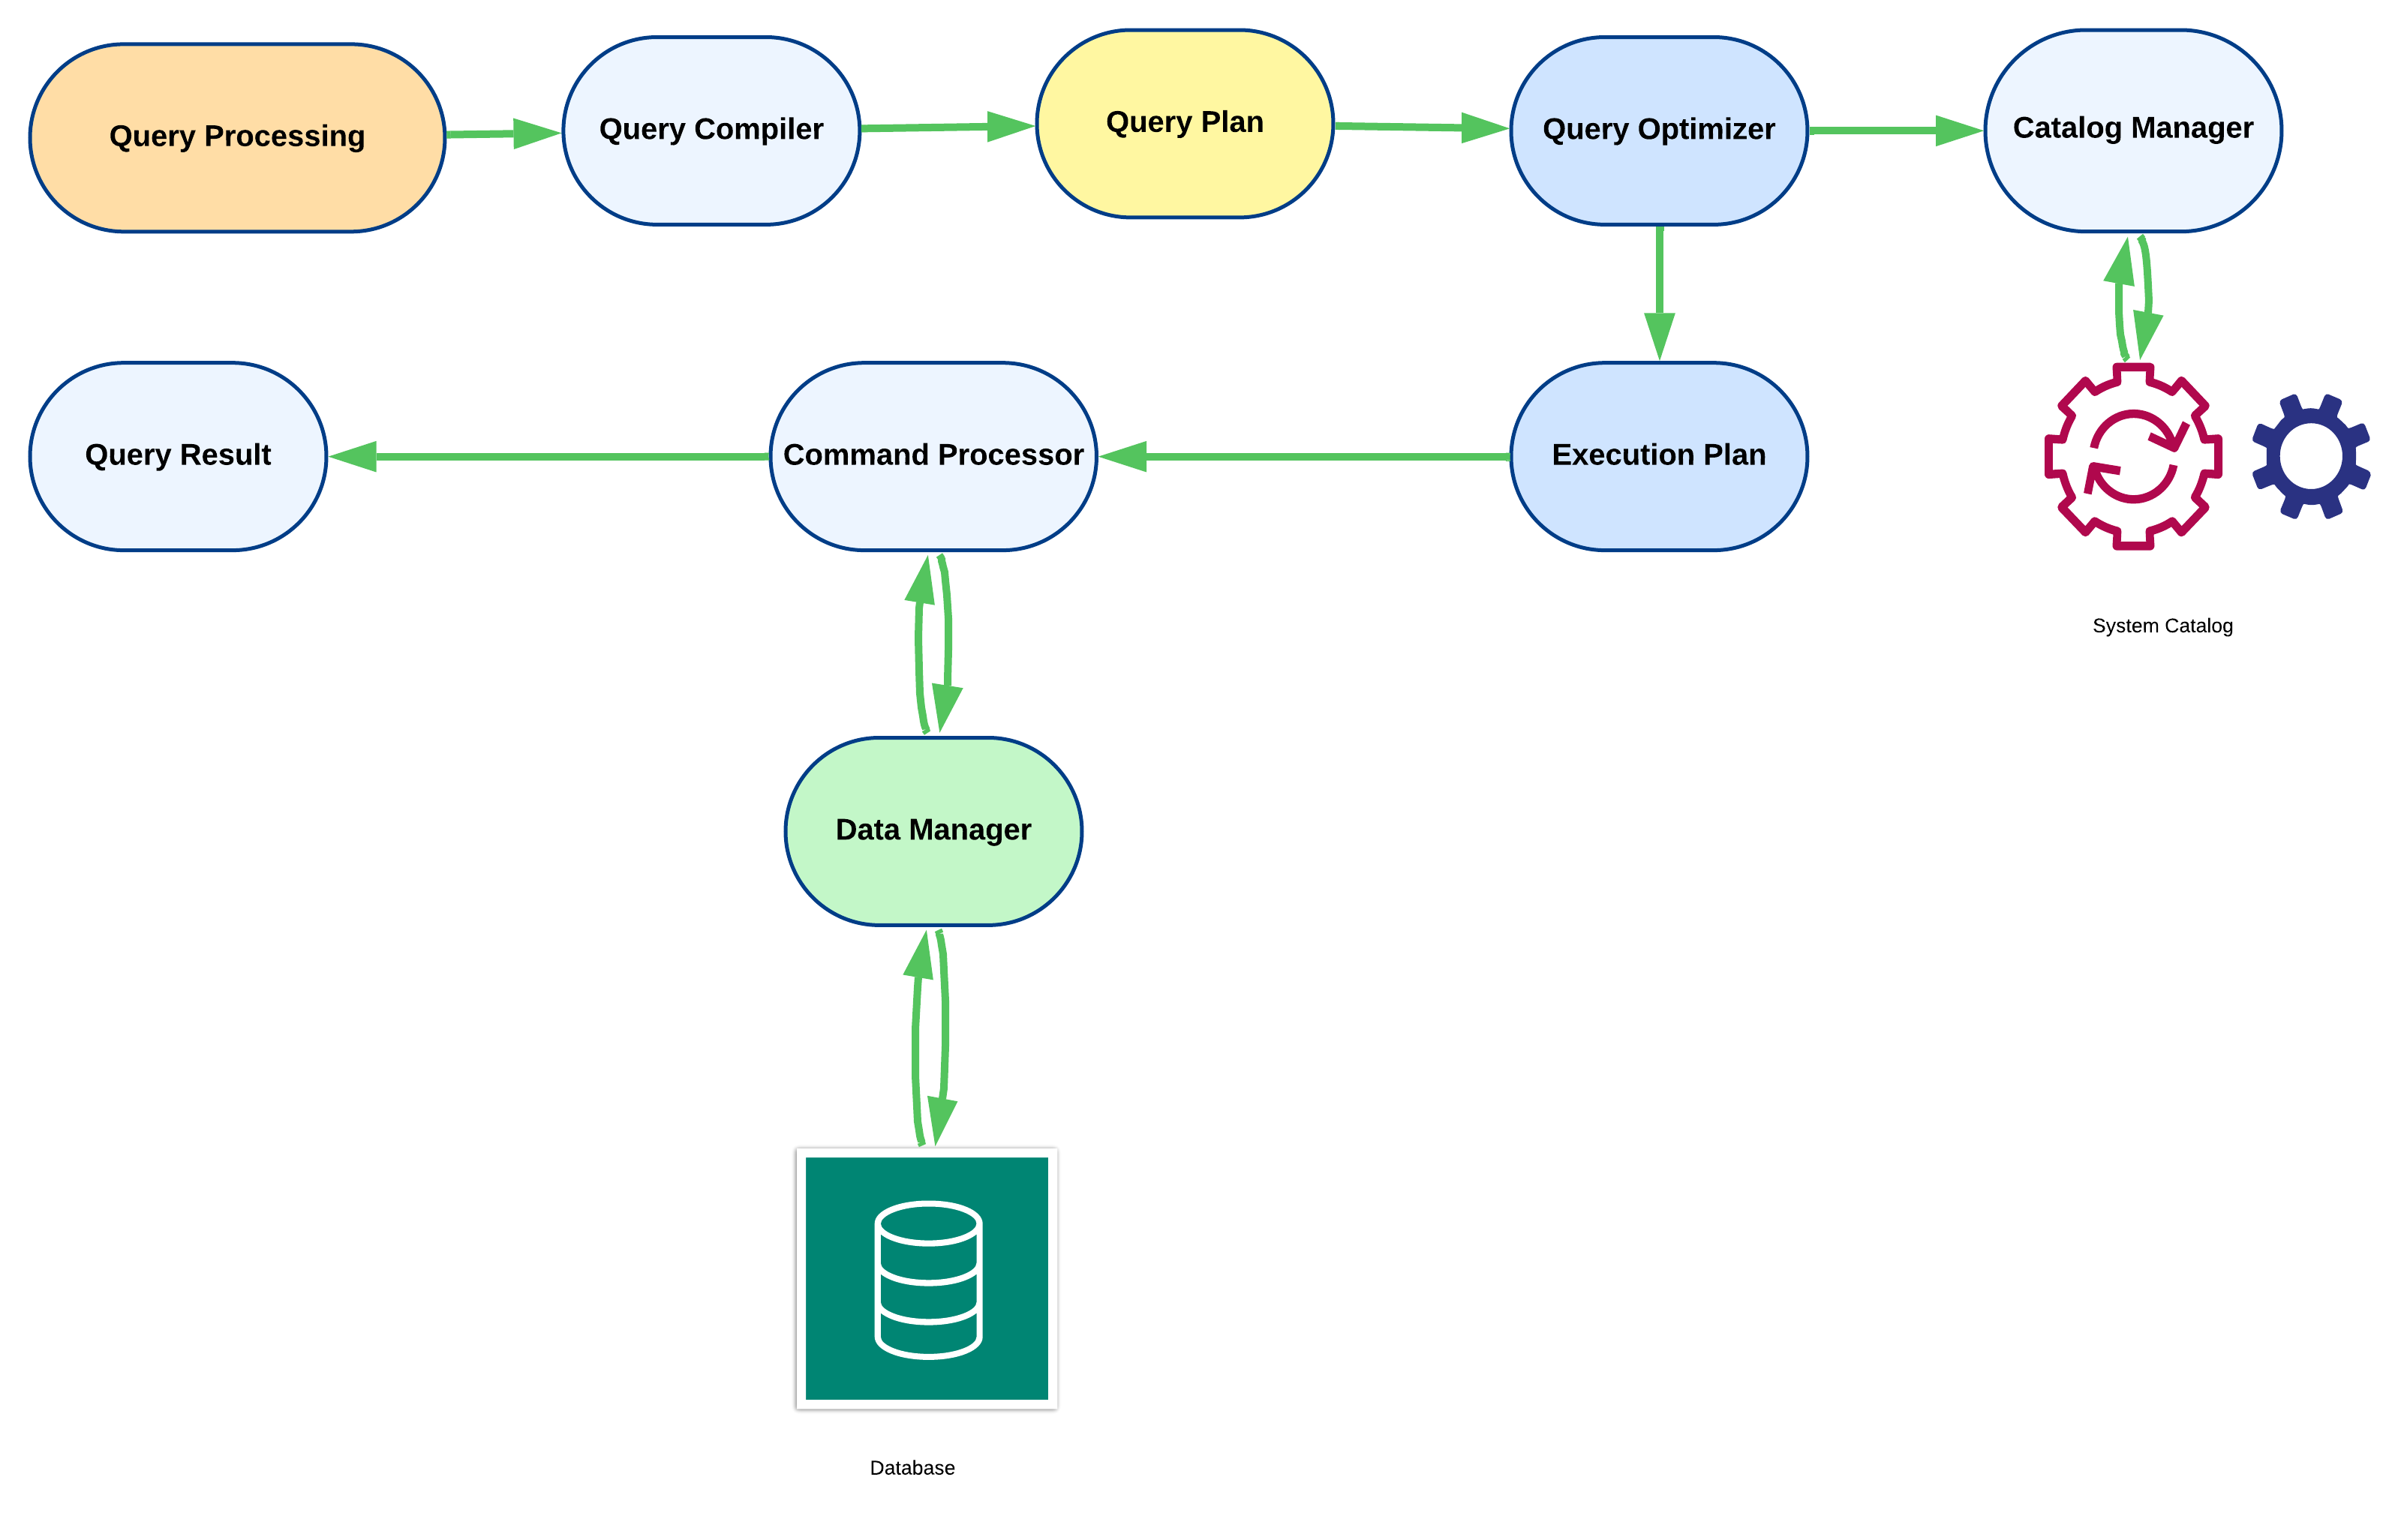
\includegraphics[width=0.5\textwidth]{Figure/Flow of query processing.png}
    \caption[The flow of query processing in DBMS]{The flow of query processing in DBMS ~\cite{wwwnaukricom-no-date} }
     
    \label{fig:my_image} 
\end{figure}
\begin{enumerate}
\item \textbf{Parser:} Query parsing is the first step in query processing. In this step, the database analyzes and breaks down SQL queries by checking syntax and semantics before it is executed by the database engine\cite{wwwnaukricom-no-date}.

    \begin{enumerate}
        \item \textbf{Syntax check:} Syntax validation is the process of validating the structure and format of a query to ensure its functionality and adherence to the SQL language rules before executing it. Here is a general example of a syntax error. \vspace{.4cm}
        
        % Define colors
\definecolor{codegreen}{rgb}{0,0.6,0}  % Green for comments
\definecolor{codegray}{rgb}{0.5,0.5,0.5}  % Gray for numbers
\definecolor{codepurple}{rgb}{0.58,0,0.82}  % Purple for strings
\definecolor{backcolour}{rgb}{0.95,0.95,0.92}  % Light gray background
\definecolor{bordercolor}{rgb}{0.7,0.7,0.7}  % Left border color (gray)
\definecolor{codeblue}{rgb}{0,0,0.8}  % Blue for SQL keywords

\lstdefinelanguage{MySQL}{
    keywords={SELECT, FROM, WHERE, JOIN, ON, INNER, OUTER, LEFT, RIGHT, FULL, GROUP, BY, ORDER, ASC, DESC, AS, COUNT, SUM, AVG, MAX, MIN, DISTINCT, INSERT, INTO, VALUES, UPDATE, SET, DELETE, CREATE, TABLE, PRIMARY, FOREIGN, KEY, DEFAULT, NULL, NOT, CHECK, CONSTRAINT, INDEX, VIEW, MATERIALIZED, PROCEDURE, FUNCTION, TRIGGER, DATABASE, ALTER, DROP, EXEC, IF, EXISTS, UNION, ALL, CASE, WHEN, THEN, ELSE, END, CAST, CONVERT, LIKE, IN, BETWEEN, AND, OR, HAVING, LIMIT, OFFSET},
    sensitive=false,
    morestring=[b]',  % String in single quotes
    morestring=[b]"   % String in double quotes
}
\captionsetup[lstlisting]{font=small}
\lstdefinestyle{sqlstyle}{
    backgroundcolor=\color{backcolour},   
    commentstyle=\color{codegreen},  % Comments in green
    keywordstyle=\bfseries\color{codeblue},  % ✅ SQL Keywords in Blue & Bold
    numberstyle=\scriptsize\color{codegray},  % Row numbers in gray
    stringstyle=\color{codepurple},  % Strings in purple
    basicstyle=\ttfamily\footnotesize,
    breaklines=true,
    captionpos=b,
    numbers=left,      % ✅ Enables row numbers on the left
    stepnumber=1,      % ✅ Row numbers increment by 1
    firstnumber=1,     % ✅ Starts numbering at 1
    numbersep=8pt,     % ✅ Increases space between numbers and SQL code
    xleftmargin=3em,   % ✅ Ensures space inside the left border
    frame=single,      % ✅ Keeps a single border (left-aligned)
    framesep=5pt,      % ✅ Ensures space inside the frame
    rulesepcolor=\color{bordercolor},  % ✅ Matches row numbers with left border
    rulecolor=\color{bordercolor},  % ✅ Sets left border color
    language=MySQL  % ✅ Uses SQL keyword highlighting
}



\begin{lstlisting}[style=sqlstyle, caption={SQL query to check syntax}]
SQL>SELECT * form employees;SELECT * form employees * error at line 1:
FROM   keyword NOT found
WHERE  expected
\end{lstlisting}
        
          Here, the error of the wrong spelling of FROM is given by this check.\vspace{.4cm}
          
        \item \textbf{Semantic check:} It checks whether the statement is meaningful or not. Example: Query contains a table name which does not exist.
        
        
\definecolor{dkgreen}{rgb}{0,0.6,0}
\definecolor{gray}{rgb}{0.5,0.5,0.5}
\definecolor{mauve}{rgb}{0.58,0,0.82}
\lstset{language=SQL,
  basicstyle={\small\ttfamily},
  belowskip=3mm,
  breakatwhitespace=true,
  breaklines=true,
  classoffset=0,
  columns=flexible,
  commentstyle=\color{dkgreen},
  framexleftmargin=0.25em,
  frameshape={}{yy}{}{}, %To remove to vertical lines on left, set `frameshape={}{}{}{}`
  keywordstyle=\color{blue},
  numbers=none, %If you want line numbers, set `numbers=left`
  numberstyle=\tiny\color{gray},
  showstringspaces=false,
  stringstyle=\color{mauve},
  tabsize=3,
  xleftmargin =1em
}
         \begin{lstlisting}
         SQL> SELECT * FROM nonexistent_table;
         SELECT * FROM nonexistent_table
              *
        ERROR at line 1:
        ORA-00942: table or view does not exist
        FROM keyword not found where expected
        \end{lstlisting}
        
        A syntactically correct statement can fail a semantic check, as shown in the above example of a query of a nonexistent table \cite{Oracle}.\vspace{.4cm}
        
        \item \textbf{Shared pool check:} During the parse, the database performs a shared pool check to determine whether it can skip (hash code)\footnote{The hashCode() method is used to generate the hash values of objects.} resource-intensive steps of statement processing. Every query possesses a hash code.\vspace{.4cm}
        
        % Define colors
\definecolor{codegreen}{rgb}{0,0.6,0}  % Green for comments
\definecolor{codegray}{rgb}{0.5,0.5,0.5}  % Gray for numbers
\definecolor{codepurple}{rgb}{0.58,0,0.82}  % Purple for strings
\definecolor{backcolour}{rgb}{0.95,0.95,0.92}  % Light gray background
\definecolor{bordercolor}{rgb}{0.7,0.7,0.7}  % Left border color (gray)
\definecolor{codeblue}{rgb}{0,0,0.8}  % Blue for SQL keywords

\lstdefinelanguage{MySQL}{
    keywords={SELECT, FROM, WHERE, JOIN, ON, INNER, OUTER, LEFT, RIGHT, FULL, GROUP, BY, ORDER, ASC, DESC, AS, COUNT, SUM, AVG, MAX, MIN, DISTINCT, INSERT, INTO, VALUES, UPDATE, SET, DELETE, CREATE, TABLE, PRIMARY, FOREIGN, KEY, DEFAULT, NULL, NOT, CHECK, CONSTRAINT, INDEX, VIEW, MATERIALIZED, PROCEDURE, FUNCTION, TRIGGER, DATABASE, ALTER, DROP, EXEC, IF, EXISTS, UNION, ALL, CASE, WHEN, THEN, ELSE, END, CAST, CONVERT, LIKE, IN, BETWEEN, AND, OR, HAVING, LIMIT, OFFSET},
    sensitive=false,
    morestring=[b]',  % String in single quotes
    morestring=[b]"   % String in double quotes
}

\lstdefinestyle{sqlstyle}{
    backgroundcolor=\color{backcolour},   
    commentstyle=\color{codegreen},  % Comments in green
    keywordstyle=\bfseries\color{codeblue},  % ✅ SQL Keywords in Blue & Bold
    numberstyle=\scriptsize\color{codegray},  % Row numbers in gray
    stringstyle=\color{codepurple},  % Strings in purple
    basicstyle=\ttfamily\footnotesize,
    breaklines=true,
    captionpos=b,
    numbers=left,      % ✅ Enables row numbers on the left
    stepnumber=1,      % ✅ Row numbers increment by 1
    firstnumber=1,     % ✅ Starts numbering at 1
    numbersep=8pt,     % ✅ Increases space between numbers and SQL code
    xleftmargin=3em,   % ✅ Ensures space inside the left border
    frame=single,      % ✅ Keeps a single border (left-aligned)
    framesep=5pt,      % ✅ Ensures space inside the frame
    rulesepcolor=\color{bordercolor},  % ✅ Matches row numbers with left border
    rulecolor=\color{bordercolor},  % ✅ Sets left border color
    language=MySQL  % ✅ Uses SQL keyword highlighting
}



\begin{lstlisting}[style=sqlstyle, caption={SQL query to check shared pool}]
     ALTER SESSION SET OPTIMIZER_MODE=ALL_ROWS;
     ALTER SYSTEM FLUSH SHARED_POOL; 
     SELECT * FROM Employees WHERE DepartmentID = 10;

\end{lstlisting}
        
        In this example, When the \textbf{SELECT} statement is executed, the SQL server checks the plan cache to see if an execution plan for this identical query already exists. If a matching execution plan is found in the cache\footnote{A cache in SQL is a high-speed data storage layer that temporarily stores frequently accessed data to improve query performance and reduce database load} (a ``cache hit''), SQL server reuses it, allowing for quicker execution without going through the parsing and optimization steps again.
        
    \end{enumerate}
    
%\begin{figure}[h]
   % \centering
   % 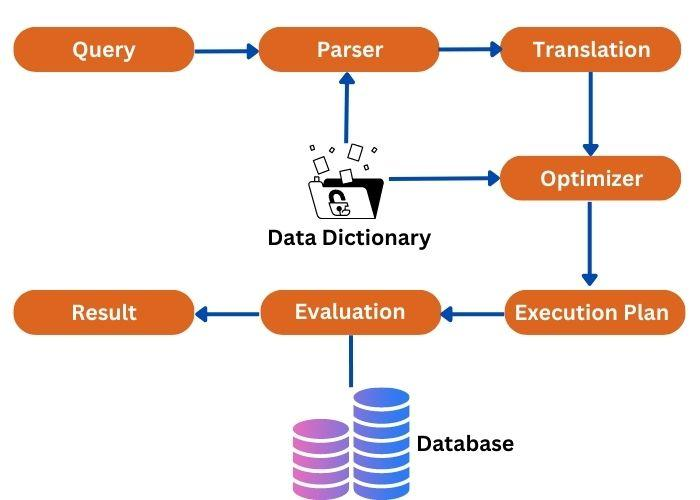
\includegraphics[width=0.5\textwidth]{Figure/Query processing.jpg}
   % \caption[The flow of query processing in DBMS]{The flow of query processing in DBMS \cite{Oracle}}
    %\label{fig:my_image}
%\end{figure}
    
    \item \textbf{Optimizer}: After parsing the query, the DBMS starts to find the most efficient way of executing the provided query. The factors for the query follow some optimization process. During the optimization stage, at least one complex parsing of one unique DML\footnote{DML  (data manipulation language) refers to a computer programming language that allows you to add (insert), delete (delete), and alter (update) data in a database.} statement must be done. The database never optimizes DDL\footnote{Data definition or data description language (DDL) is a syntax for creating and modifying database objects such as tables, indices, and users.} unless it includes a DML component, such as a sub-query, which needs optimization. Such operations are used for selecting data, inserting something, and updating. After everything is completed, then the evaluation step is made. In this step, the DBMS returns the result.
    
    \item \textbf{Result:} After getting the best execution plan, the DBMS starts the execution of the optimized query and operates on data, including selecting the data, inserting something, and updating the data. Once everything is completed, DBMS returns the result after the evaluation step \cite{Query,QueryProcessing,Oracle}.
    
\end{enumerate}

\subsection{Query Optimization } Code is written with the goal of optimal logic in terms of both space and time complexity. Likewise, when database queries are written, they are desired to be optimal in terms of their execution time and resource utilization. Query optimization is a crucial aspect of DBMS that seeks the most efficient way to execute a given query by considering a variety of query execution strategies. It minimizes the total cost or the total response time for the execution of a query. It is one of the key factors that affect the application performance.\vspace{.4cm}

The result of a query is generated by processing the rows and columns in a database in a way that yields the requested information. Since database structures are complex, in most cases, and especially for not very simple queries, the needed data for a query can be collected from a database by accessing it in different ways through different data structures and in different orders \cite{selinger-1979}. Each different method usually requires varying processing times. The time it takes to process the same query can vary significantly, ranging from a fraction of a second to hours, depending on the selected method. The goal of query optimization is to determine how to process a given query in the shortest time possible. The significant potential variance in processing time justifies the need for query optimization. However, identifying the exact optimal query plan from all available options is often very complex, time-consuming, and frequently impractical. Therefore, query optimization generally aims to approximate the optimum by evaluating several reasonable alternatives to deliver results within an acceptable time frame. \vspace{.4cm}

There is a trade-off between the amount of time spent figuring out the best query plan and the quality of the choice, and the optimizer may not choose the best answer on its own. Database management systems have different qualities and ways of balancing these two. Cost-based query optimizes and evaluates the resource footprints of various query plans and uses this as the basis for plan selection. These assign an estimated cost to each possible query plan and choose the plan with the smallest cost. Cost is used to estimate the runtime cost of evaluating the query in terms of the number of I/O operations required, CPU path length, amount of disk buffer space, disk storage service time, and connection consumption between units of parallelism, and other factors identified from the data directory. The set of query strategies is formed by examining the possible access paths, e.g., primary index, secondary index access, full file scan, and various relational table join techniques, e.g., Merge join, has join, and Product join. The search space can become quite large depending on the complexity of the SQL query. There are two types of optimization. These consist of logical optimization, which generates a sequence of relational algebra to solve the query, and physical optimization, which is used to determine the means of carrying out each operation \cite{dremio-2024}.\vspace{.4cm}

Query optimization is crucial for databases to enhance efficiency and performance. It enables organizations to significantly increase query speed, decrease data retrieval times, and minimize resource usage. By doing this, it not only identifies and addresses issues like slow queries and bottlenecks but also ensures that the database operates at its best, delivering faster and more reliable data processing. Ultimately, effective optimization results in a better user experience and heightened productivity throughout the organization\cite{team-2023, r-2024}.


\subsubsection{Database Query Performance Metrics}
The following metrics play a vital role in effectively measuring the performance of SQL queries. However, most relevant metrics may vary depending on the specific database system and application requirements.
Here is a summary of key metrics used to evaluate and enhance query performance \cite{chwesewicz-2024}.
\begin{itemize}
    \item\textbf{Query execution time}: Query execution time refers to the duration it takes for a database to process and return results for a given SQL query. Measured in seconds or milliseconds. Lower execution time indicates better performance.
    \item\textbf{Query throughput}: It measures the number of queries or operations a database can handle per unit of time, typically expressed as transactions per second (TPS) and queries per second(QPS).
    \item\textbf{Resource utilization}: Measures the percentage of time the CPU is occupied processing database operations. High CPU or memory usage can indicate a heavy processing load or un-optimized queries.
\end{itemize}

\subsubsection{Key Optimization Techniques}

Optimizing a query is critical for increasing database performance. There are various optimization strategies. However, the following are the most widely used:

 \begin{itemize}
     \item \textbf{Indexing}: Indexing is a crucial technique for query optimization in databases. It's named indexing because of how an index works in a book. An index is a structure that holds the field the index is sorting and a pointer from each record to their corresponding record in the original table where data is actually stored \cite{tomar-2021,atlassian-no-date}.
     \item \textbf{Query rewriting}: It is a technique used in query optimization to transform a given database query into an equivalent form that executes more efficiently. It is one of the initial phases of query processing, where the original query is parsed and translated into an internal representation. This method is particularly useful for complex queries, including those queries that have many sub-queries or many join \cite{pitoura-2009,unknown-IBM-25-2024}.
     
     \item \textbf{Partitioning}: This optimization method is especially effective for large databases. It involves splitting a large table or index into smaller segments to make the query more manageable pieces. Each partition acts as a separate entity that can be managed independently \cite{planck-2024}.
     
     \item \textbf{Caching:} It is a vital technique that involves storing cache results in RAM\footnote{ RAM is a form of electronic computer memory that can be read and changed in any order, typically used to store working data and machine code.} for ultra-fast access or on disk of frequently executed queries. This is particularly useful for queries that are executed across multiple requests \cite{Bit-Fetch-2024}.
     
     \item\textbf{Materialized view}: Materialized views are a powerful tool for query optimization. This paper has demonstrated the significant impact of materialized views on query optimization, highlighting their role as a crucial tool for improving database performance. A detailed explanation can be found in the \hyperref[term:materialized_views]{chapter 2.6}.\vspace{.4cm}
     
 \end{itemize}
 
 \subsection{Reasons for Using Materialized View for Query Optimization}
 Materialized views(MVs) offer several compelling reasons for query optimization in a scheduled manner without compromising accuracy or freshness. Here are some key points:
 
\begin{itemize}
    \item\textbf{Precomputed result:} Materialized views store the results of a query that allows subsequent queries to access these precomputed results directly rather than recalculating them from the base tables. These results are updated periodically or on-demand based on the underlying data changes \cite{khan-2023,Risingwave-no-date}.
    
    \item\textbf{Reduced Query complexity:} The main reason for creating materialized views is to improve query performance. It stores a snapshot of the data, which reduces the need for intricate query design, as we get the accesses precomputed results directly \cite{Risingwave-no-date,Databricks-no-date}.
    
    \item\textbf{Efficient use of resources:} As we get the data from pre-computed data and do not need to run a full query every time materialized views decrease the computational load on database servers. It leads to faster query response time, improved overall system performance, and requires fewer resources \cite{google-no-date, khan-2023}.
    
\end{itemize}\vspace{.4cm}

The motivation for using materialized views is to enhance performance. However, the additional effort involved in managing them can become a significant concern for system administration. Common management tasks for materialized views include identifying which views to generate, indexing them, and ensuring that all materialized views and indexes are refreshed properly whenever the database is updated. Standard management activities also involve reviewing which materialized views have been used and evaluating how effectively each view has impacted workload performance. It's also important to determine how much space materialized views occupy and which views should be removed. Outdated information should be archived, and materialized view data that is no longer useful should be deleted \cite{Ashadevi2008CostEA,1363763}.

\subsubsection{Challenges in Query Optimization} Query optimization is a crucial aspect of database management, aiming to improve the performance and efficiency of SQL queries. Opta data group, a company specializing in healthcare data management, faces several challenges with query optimization in its MSSQL environment. Given the vast amount of patient and operational data they handle, inefficient queries can lead to slow response times and increased resource consumption \cite{Flipico-2024}. The following example scenario shows query challenges:\vspace{.4cm}


% Define colors
\definecolor{codegreen}{rgb}{0,0.6,0}  % Green for comments
\definecolor{codegray}{rgb}{0.5,0.5,0.5}  % Gray for numbers
\definecolor{codepurple}{rgb}{0.58,0,0.82}  % Purple for strings
\definecolor{backcolour}{rgb}{0.95,0.95,0.92}  % Light gray background
\definecolor{bordercolor}{rgb}{0.7,0.7,0.7}  % Left border color (gray)
\definecolor{codeblue}{rgb}{0,0,0.8}  % Blue for SQL keywords

\lstdefinelanguage{MySQL}{
    keywords={SELECT, FROM, WHERE, JOIN, ON, INNER, OUTER, LEFT, RIGHT, FULL, GROUP, BY, ORDER, ASC, DESC, AS, COUNT, SUM, AVG, MAX, MIN, DISTINCT, INSERT, INTO, VALUES, UPDATE, SET, DELETE, CREATE, TABLE, PRIMARY, FOREIGN, KEY, DEFAULT, NULL, NOT, CHECK, CONSTRAINT, INDEX, VIEW, MATERIALIZED, PROCEDURE, FUNCTION, TRIGGER, DATABASE, ALTER, DROP, EXEC, IF, EXISTS, UNION, ALL, CASE, WHEN, THEN, ELSE, END, CAST, CONVERT, LIKE, IN, BETWEEN, AND, OR, HAVING, LIMIT, OFFSET},
    sensitive=false,
    morestring=[b]',  % String in single quotes
    morestring=[b]"   % String in double quotes
}

\lstdefinestyle{sqlstyle}{
    backgroundcolor=\color{backcolour},   
    commentstyle=\color{codegreen},  % Comments in green
    keywordstyle=\bfseries\color{codeblue},  % ✅ SQL Keywords in Blue & Bold
    numberstyle=\scriptsize\color{codegray},  % Row numbers in gray
    stringstyle=\color{codepurple},  % Strings in purple
    basicstyle=\ttfamily\footnotesize,
    breaklines=true,
    captionpos=b,
    numbers=left,      % ✅ Enables row numbers on the left
    stepnumber=1,      % ✅ Row numbers increment by 1
    firstnumber=1,     % ✅ Starts numbering at 1
    numbersep=8pt,     % ✅ Increases space between numbers and SQL code
    xleftmargin=3em,   % ✅ Ensures space inside the left border
    frame=single,      % ✅ Keeps a single border (left-aligned)
    framesep=5pt,      % ✅ Ensures space inside the frame
    rulesepcolor=\color{bordercolor},  % ✅ Matches row numbers with left border
    rulecolor=\color{bordercolor},  % ✅ Sets left border color
    language=MySQL  % ✅ Uses SQL keyword highlighting
}

\begin{lstlisting}[style=sqlstyle, caption={Challenges in query optimization}]
SELECT *
FROM   patients
       JOIN treatments
         ON patients.patientid = treatments.patientid
WHERE  treatmentdate >= '2024-12-02'; 
\end{lstlisting}


The join condition in the above query relates the two tables, namely `` Patients '' and `` Treatment ''. Suppose the `` PatientID '' column in both the ``Patients'' and `` Treatment'' tables is not indexed properly. In that case, the database may perform a full table scan, and that might happen when only a few columns are required from a very big table, and this would cause very slow response times and a lot of resources consumed. Further details about the key challenges during query optimization are discussed below:

\begin{itemize}
    \item\textbf{Data Fragmentation and Localization}: Dealing with how data is partitioned and distributed across multiple nodes. Data can be fragmented both horizontally and vertically and spread across nodes. Balancing between local execution and data transfer is also challenging. 
    \item\textbf{Query Decomposition and Allocation}: It refers to the process of breaking down a query into sub-queries and assigning them to different nodes. It is challenging to choose the best sub-queries and nodes.
    \item\textbf{Complexity of Query Execution Plans}: Query optimization involves various techniques. Mastering these techniques can be challenging in finding the most efficient one, especially for complex or multi-table queries.
    \item\textbf{Dependency on Indexes}: Proper indexing improves query performance, but failing to create or maintain supporting indexes can result in inefficient query executions. Managing and updating indexes as data grows and changes can become a challenge Expressed during optimization as a cost function. The common choice is to minimize response time within given resource limitations.\cite{team-2020,etutorials-03-2024,editor-ijmter-2015}.
\end{itemize}

During the experiment, there were numerous challenges encountered, as mentioned above. It was challenging to split materialized views across multiple nodes and minimize data transfer costs due to data fragmentation. It was not straightforward to divide queries into sub-queries and split them into nodes to get the best execution efficiency. Query execution plans were complicated with joins between multiple tables and aggregations, and it was challenging to decide the best way to execute them. In addition, proper indexing was necessary to maintain query performance since the absence of creating or updating indexes resulted in inefficient execution. The PSO algorithm avoids all these complexities since it minimizes the cost function to obtain minimum response time and resource consumption. 

\subsubsection*{Optimization Goals}

\begin{itemize}
    \item Minimize response time
    \item Minimize resource consumption
    \item Minimize time to the first tuple
    \item Maximize throughput
\end{itemize}\vspace{.4cm}

This paper shares the same optimization goals, particularly focusing on minimizing response time. The primary objective is to enhance query performance by limiting execution latency and minimizing resource consumption and time to the first tuple. Maximizing throughput is also considered to enable efficient handling of multiple queries. By using materialized views and the PSO algorithm, this work aims to accomplish all these goals, with an emphasis on optimizing response time to improve query execution more quickly.



\subsection{What is a View in SQL}
A view in SQL is a virtual table that is generated by an SQL query. It does not store data physically but retrieves it from the underlying base table. Views are compiled at runtime, and they simplify the presentation of data from one or more tables without modifying the original data. It can be made over one or more database tables. Generally, those columns that need to be queried repeatedly are put into a view. Once the view is created, an index can be made, the view can be triggered, and the view can be queried as a table. The view can function as a filter for specific tables it references \cite{chauhan-2024, Rohan_Vats-2024}.\vspace{.4cm}

A view is a component of a database that provides a specific user with an impression of data while restricting access to the original database tables. In this context, the original tables are known as view tables. A view can represent data from a database, facilitate a specific selection of data, or compute new data that reflects the contents of the underlying base tables. In other words, every analytical operation derived from the base table data originates from a view table.\vspace{.4cm}




The following example explains the concept of view:


\definecolor{dkgreen}{rgb}{0,0.6,0}
\definecolor{gray}{rgb}{0.5,0.5,0.5}
\definecolor{mauve}{rgb}{0.58,0,0.82}
\lstset{language=SQL,
  basicstyle={\small\ttfamily},
  belowskip=3mm,
  breakatwhitespace=true,
  breaklines=true,
  classoffset=0,
  columns=flexible,
  commentstyle=\color{dkgreen},
  framexleftmargin=0.25em,
  frameshape={}{yy}{}{}, %To remove to vertical lines on left, set `frameshape={}{}{}{}`
  keywordstyle=\color{blue},
  numbers=none, %If you want line numbers, set `numbers=left`
  numberstyle=\tiny\color{gray},
  showstringspaces=false,
  stringstyle=\color{mauve},
  tabsize=3,
  xleftmargin =1em
}
         \begin{lstlisting}
CREATE VIEW AokCustommers AS
SELECT CustomerName
FROM Customers
WHERE Country = 'Germany';
        \end{lstlisting}

 In this example, the view ``AokCustomers'' is created to simplify access to customer names, specially from Germany. This view dynamically retrieves the relevant data from the ``Customers'' table, allowing for easier and more efficient data retrieval.
 
\subsubsection{Types of Views}

There are two types of view in SQL server
\begin{itemize}
    \item \textbf{System defined view}: The system-defined views are predefined views that already exist in the master database of the SQL server, such as tempdb, master, and temp. Each of the databases has its properties and functions. These system views will be automatically attached to any user-defined database. It will expose the metadata of the database, and it can be used to get all possible information about the instance of the SQL server or database objects, columns, and contains. There are three types of System-defined views: Information Schema, Catalog View, and Dynamic Management View \cite{chauhan-2024}.
    \item \textbf{User-defined view}: These are the types of views that the user created to meet their specific requirements. It can also be divided into three types: simple, complex, and materialized views that help to organize, secure, and simplify access to database information \cite{javapoint-author-2024}.
\end{itemize}
   
\subsection{Materialized Views}\label{term:materialized_views}
\noindent\textit{Materialized views, also known as materialized tables or summary tables, are database objects that physically store the result of a query. Unlike regular views, which are virtual and compute their results on the fly, materialized views pre-compute and store the query results, allowing for faster retrieval and improved query performance.} \vspace{.3cm}

Materialized views in databases optimize query performance by pre-computing and storing the results of complex queries involving aggregations and joins. This reduces the computational load during execution, significantly speeding up response times.\vspace{.4cm}

 A special type of view is materialized views. It refers to the fact that the contents of the view are stored in the form of a separate table in the database system. MV is designed to the user's requirements. An MV definition includes aggregation functions like MIN\footnote{The MIN function returns the smallest value in a set of non-NULL values.}, MAX\footnote{The MAX function returns the largest value in a set of non-NULL values.}, COUNT(DISTINCT), COUNT(*)\footnote{COUNT returns the number of rows that match the specified criteria.}, SUM\footnote{SUM calculates the total of a set of values.}, and AVG\footnote{AVG computes the average value of a set of non-NULL values.}, one or more tables joined together, and a GROUP BY operation on attributed and basic data definition language operation such as CREATE; ALTER and DROP may be applied on tables \cite{Kardel_Thakare}. MV is a decision support/ data warehousing system tool that can increase the speed of queries that access a large number of records by many orders of magnitude \cite{Kishan_Sainath_no_date}. Nevertheless, materialized views can also be stored as a file or a data structure in memory. In addition to that, a virtual view would be loaded from the base table when requested. While the on-demand idea behind virtual views is certainly desirable \cite{jan-no-date,ashadevi-2024}.\vspace{.4cm}



A materialized view (sometimes called a sorted, projected and materialized view or SPM view) is a view whose columns have been sorted, projected and materialized.\cite{IBM} In database systems, optimize query performance by pr-computing and storing the result of complex queries involving aggregations and joins. As they store the results physically in a table, re-computation of a query is not needed again. When the view is already materialized at any time, the same query is entered into the system. This reduces the computational load during the execution, significantly speeding up the response times.\vspace{.4cm}

\subsubsection{Working Principle of Materialized Views}
The working principle of MV can be described as follows:

\begin{itemize}
    \item\textbf{Pre-computations:} It stores the results of queries that involve complex join and aggregations. These results are pre-computed and stored in the database, reducing the time needed to fetch the data when required.
    \item\textbf{Storage and retrieval:} The data in a materialized view is periodically refreshed to reflect changes in the underlying tables. The refresh can be scheduled or triggered by specific events, depending on the use case and requirements.
    \item\textbf{Refresh mechanism:}  Materialized views need to be refreshed to stay up to date with the underlying data.\vspace{.4cm}

    \begin{itemize}
        \item\textbf{Full Refresh:} The entire view is recomputed from scratch.
        \item\textbf{Incremental Refresh:} Only the changes since the last refresh are applied.
        \item\textbf{On Demand Refresh:} Triggered by specific events or user requests.
    \end{itemize}
 
\end{itemize}\vspace{.4cm}

Materialized views must be refreshed every now and then to maintain synchrony with the base information. This research employs the on-demand refresh mechanism among several strategies used. The on-demand refresh strategy updates the materialized view when specific events or user requests happen. The on-demand refresh strategy is employed in this research due to its flexibility and ability to save resources while allowing targeted updates when precision in data is critical.

\subsubsection{Types of Materialized Views}
The most prevalent forms of materialized views in database management systems are:

\vspace{.4cm}

\begin{enumerate}[label=\alph*)]
 \item\textbf{ Materialized views with aggregates:} Materialized views with aggregates store the results of queries that perform aggregate calculations (e.g., SUM, COUNT, AVG, MIN, MAX) over large datasets. These views are particularly useful for optimizing query performance in scenarios that involve complex aggregations over vast amounts of data, such as reporting, analytics, and decision support systems. The explanation is demonstrated with the following example:\vspace{.4cm}
    
    
\definecolor{dkgreen}{rgb}{0,0.6,0}
\definecolor{gray}{rgb}{0.5,0.5,0.5}
\definecolor{mauve}{rgb}{0.58,0,0.82}
\lstset{language=SQL,
  basicstyle={\small\ttfamily},
  belowskip=3mm,
  breakatwhitespace=true,
  breaklines=true,
  classoffset=0,
  columns=flexible,
  commentstyle=\color{dkgreen},
  framexleftmargin=0.25em,
  frameshape={}{yy}{}{}, %To remove to vertical lines on left, set `frameshape={}{}{}{}`
  keywordstyle=\color{blue},
  numbers=none, %If you want line numbers, set `numbers=left`
  numberstyle=\tiny\color{gray},
  showstringspaces=false,
  stringstyle=\color{mauve},
  tabsize=3,
  xleftmargin =1em
}
         \begin{lstlisting}
 
CREATE MATERIALIZED VIEW SalesSummary
AS
SELECT
    ProductID,
    Region,
    CategoryID,
    SUM(SalesAmount) AS TotalSales,
    AVG(SalesAmount) AS AvgSales,
    COUNT(*) AS NumberOfSales
FROM Sales
GROUP BY ProductID, Region, CategoryID;

        \end{lstlisting}

    In this example, the materialized view ``salesSummary'' precomputes the SUM, AVG, and COUNT for sales data grouped by ProductID, Region, and CategoryID.

    \item\textbf{Materialized views with join }: Materialized views with joins store the results of queries that involve multiple tables combined using join operations (e.g., INNER JOIN, LEFT JOIN, RIGHT JOIN). These types of materialized views can significantly speed up complex queries that frequently access multiple related tables. By precomputing the join results, the materialized view avoids the need to recompute them during every query execution. The explanation is made clear with the following example: \vspace{.4cm}
    
    
\definecolor{dkgreen}{rgb}{0,0.6,0}
\definecolor{gray}{rgb}{0.5,0.5,0.5}
\definecolor{mauve}{rgb}{0.58,0,0.82}
\lstset{language=SQL,
  basicstyle={\small\ttfamily},
  belowskip=3mm,
  breakatwhitespace=true,
  breaklines=true,
  classoffset=0,
  columns=flexible,
  commentstyle=\color{dkgreen},
  framexleftmargin=0.25em,
  frameshape={}{yy}{}{}, %To remove to vertical lines on left, set `frameshape={}{}{}{}`
  keywordstyle=\color{blue},
  numbers=none, %If you want line numbers, set `numbers=left`
  numberstyle=\tiny\color{gray},
  showstringspaces=false,
  stringstyle=\color{mauve},
  tabsize=3,
  xleftmargin =1em
}
         \begin{lstlisting}
CREATE MATERIALIZED VIEW CustomerOrderSummary
AS
SELECT
    c.CustomerID,
    c.CustomerName,
    o.OrderID,
    o.OrderDate,
    p.ProductID,
    p.ProductName,
    o.Quantity,
    o.TotalAmount
FROM
    Customers c
JOIN
    Orders o ON c.CustomerID = o.CustomerID
JOIN
    Products p ON o.ProductID = p.ProductID;

        \end{lstlisting}

    In this example, the materialized view ``CustomerOrderSummary''
    stores the results of the joins between the customers, orders and products table.
    
    \item \textbf{Hybrid materialized views}: Hybrid materialized views combine features of both aggregates and join-based materialized views, optimizing performance for queries that require both aggregations and joins between multiple tables. They are designed to handle more complex queries efficiently, as they store pre-computed results that involve both aggregated data and joined tables. Hybrid materialized views are particularly useful in environments like data warehouses or reporting systems where queries often need to summarize and relate data from various sources. \vspace{.4cm}
    
    \definecolor{codegreen}{rgb}{0,0.6,0}  % Green for comments
\definecolor{codegray}{rgb}{0.5,0.5,0.5}  % Gray for numbers
\definecolor{codepurple}{rgb}{0.58,0,0.82}  % Purple for strings
\definecolor{backcolour}{rgb}{0.95,0.95,0.92}  % Light gray background
\definecolor{bordercolor}{rgb}{0.7,0.7,0.7}  % Left border color (gray)
\definecolor{codeblue}{rgb}{0,0,0.8}  % Blue for SQL keywords

\lstdefinelanguage{MySQL}{
    keywords={SELECT, FROM, WHERE, JOIN, ON, INNER, OUTER, LEFT, RIGHT, FULL, GROUP, BY, ORDER, ASC, DESC, AS, COUNT, SUM, AVG, MAX, MIN, DISTINCT, INSERT, INTO, VALUES, UPDATE, SET, DELETE, CREATE, TABLE, PRIMARY, FOREIGN, KEY, DEFAULT, NULL, NOT, CHECK, CONSTRAINT, INDEX, VIEW, MATERIALIZED, PROCEDURE, FUNCTION, TRIGGER, DATABASE, ALTER, DROP, EXEC, IF, EXISTS, UNION, ALL, CASE, WHEN, THEN, ELSE, END, CAST, CONVERT, LIKE, IN, BETWEEN, AND, OR, HAVING, LIMIT, OFFSET},
    sensitive=false,
    morestring=[b]',  % String in single quotes
    morestring=[b]"   % String in double quotes
}

\lstdefinestyle{sqlstyle}{
    backgroundcolor=\color{backcolour},   
    commentstyle=\color{codegreen},  % Comments in green
    keywordstyle=\bfseries\color{codeblue},  % ✅ SQL Keywords in Blue & Bold
    numberstyle=\scriptsize\color{codegray},  % Row numbers in gray
    stringstyle=\color{codepurple},  % Strings in purple
    basicstyle=\ttfamily\footnotesize,
    breaklines=true,
    captionpos=b,
    numbers=left,      % ✅ Enables row numbers on the left
    stepnumber=1,      % ✅ Row numbers increment by 1
    firstnumber=1,     % ✅ Starts numbering at 1
    numbersep=8pt,     % ✅ Increases space between numbers and SQL code
    xleftmargin=3em,   % ✅ Ensures space inside the left border
    frame=single,      % ✅ Keeps a single border (left-aligned)
    framesep=5pt,      % ✅ Ensures space inside the frame
    rulesepcolor=\color{bordercolor},  % ✅ Matches row numbers with left border
    rulecolor=\color{bordercolor},  % ✅ Sets left border color
    language=MySQL  % ✅ Uses SQL keyword highlighting
}

\begin{lstlisting}[style=sqlstyle, caption={Hybrid materialized views}]

CREATE materialized VIEW productsalessummary
AS SELECT r.regionname,
          p.categoryid,
          p.productname,
          c.customerid,
          SUM(o.quantity)    AS TotalQuantity,
          SUM(o.totalamount) AS TotalSales
   FROM   customers c
          join orders o
            ON c.customerid = o.customerid
          join products p
            ON o.productid = p.productid
          join regions r
            ON c.regionid = r.regionid
   GROUP  BY r.regionname,
             p.categoryid,
             p.productname,
             c.customerid; 

\end{lstlisting} 
    
This materialized view, ``ProductSalesSummary'' stores precomputed join results between customers, orders, products, and regions, as well as aggregate data on the total quantity and total sales.
    
\end{enumerate}

This paper uses materialized views with aggregates for query optimization using the PSO algorithm. Materialized views with aggregates precompute and store summarized data, such as sums, averages, and counts, which avoids significant query execution time by preventing on-the-fly computations. This method is extremely efficient for analytical query optimization and response time improvement.

Materialized views and hybrid materialized views have not been utilized in this paper because they introduce additional complexity when it comes to maintaining data consistency and require greater storage space. Materialized joins are suitable to be utilized to speed up complex joins but can introduce higher maintenance cost and more data transfer in the distributed system. Hybrid materialized views join and aggregate, but because of their complexity, they are not as well-suited to the performance goals of this research. Aggregated materialized views were therefore chosen for their simplicity and effectiveness in query execution time minimization.

\subsubsection{Materialized View vs Database View} With the usual syntax of creating a view, we create a database view, which is different from the materialized view because a normal database view is just a virtual table that is defined by a SQL query. It is stored in the user database and can be accessed by users who have appropriate permissions. An MV view does not store any data itself; it is simply a way of presenting data from one or more tables in different ways. Materialized views are disk-based and are updated periodically based on the query definition \cite{Stackoverflow-author-08-2008}. Views are virtual and run the query definition each time they are accessed. Materialized views are useful when data is accessed frequently and updated infrequently.

\subsection{Algorithm Related to the Query Optimization }
Query optimization algorithms are the methods that the database system uses to generate and select the best query execution plan for a given query. Several algorithms are commonly used to address the complex challenge of finding optimal query execution plans, including heuristic-based, cost-based, and rule-based. Heuristic-based uses predefined rules and guidelines to guide the query process, cost-based evaluates multiple execution plans and chooses the one with the lowest estimated cost, while rule-based optimization applies a fixed set of predefined rules to transform queries without considering actual data statistics. In this paper, the focus is on a cost-based algorithm like the particle swarm optimization approach, as it provides more accurate and efficient complex search spaces and converges optimal query plans.

\subsubsection{Particle Swarm Optimization Algorithm}
Particle swarm optimization is a type of optimization algorithm that depends quite on the behavior of natural organisms, such as birds or fish, that move together to achieve a common goal. A group of particles navigates the problem solution space in search of the best possible solution. Each particle adjusts its position in accordance with its best-known solution (personal best)\footnote{$P_Best$ known as local best position among all the particles.} as well as the best solution discovered by the entire group (global best)\footnote{$G_Best$ known as global best position among all the particles.}. This allows particles to converge on ideal solutions across iterations \cite{subhasis-2023}.\vspace{.4cm}

 In the case of query optimization, this makes use of all such aspects in order to optimize the configuration view, index, or query execution plan with minimum query response and resource usage in the database management systems. Here, PSO represents solution(s) as particles, for example, combinations of materialized views, which move through the solution space according to their own experiences and the swarm's experiences. By constantly changing the position of such particles, PSO iteratively finds the best optimal\footnote{Best optimal emphasizes that the solution is not just optimal (i.e., a good solution) but is the best among all possible optimal solutions found during the optimization process.} solution or near-optimum solution that has the best trade-off between query and costs of maintenance and hence becomes a very powerful means for database administrators keen on optimizing very complex database environments. Two main equations are involved in the process of PSO algorithm:\vspace{.4cm}
\begin{itemize}
    \item \textbf{Velocity update:} In this step, each particle in the swarm updates its velocity using the computed values of the individual and global best solutions and its current best position. 

\begin{equation}
v_i(t+1) = W \cdot v_i(t) + c_1 \cdot r_1 \cdot (P_Best_i - x_i(t)) + c_2 \cdot r_2 \cdot (G_Best - x_i(t))
\end{equation}

\textbf{Where:}
\begin{itemize}
    \item \( v_i(t) \): Current velocity of particle \( i \) at time \( t \).
    \item \( W \): Inertia weight that controls the influence of the previous velocity on the current velocity.
    \item \( c_1 \): Cognitive coefficient representing the weight given to the particle's own experience (personal best).
    \item \( r_1 \): A random number uniformly distributed between 0 and 1, introducing stochastic behavior.
    \item \( G_ Best_i \): The personal best position that particle \( i \) has encountered so far.
    \item \( x_i(t) \): Current position of particle \( i \) at time \( t \).
    \item \( c_2 \): Social coefficient representing the weight given to the global best position found by any particle in the swarm.
    \item \( r_2 \): Another random number uniformly distributed between 0 and 1.
    \item \( P_Best \): The global best position found by any particle in the swarm.
\end{itemize}



    The acceleration factor of the c1 and c2 coefficients is related to individual and social aspects. It determines how much confidence a particle has in itself and its neighbors to find an optimal solution \cite{baeldung2024pso}
    
    \item \textbf{Position update:} In this part, a new location of the particle is updated using the newly calculated velocity. This movement allows the particle to explore within the search space based on both its previous position and the velocity defined by its own experience and that of the swarm. The parameters of position and velocity are co-dependent.
    
    
\begin{equation}
x_i(t+1) = x_i(t) + v_i(t+1)
\end{equation}

\textbf{Where:}
\begin{itemize}
    \item \( x_i(t) \): Current position of particle \( i \) at time \( t \).
    \item \( v_i(t+1) \): Updated velocity of particle \( i \) at time \( t+1 \).
    \item \( x_i(t+1) \): New position of particle \( i \) at the next time step.
\end{itemize}

%\textbf{Description:} The position update equation states that the new position of a particle is calculated by adding its updated velocity to its current position. This movement allows the particle to explore the search space based on both its previous position and the velocity determined by its own experience and that of the swarm.



\end{itemize} 

\textbf{Example Scenario:} Consider a scenario where a company has a database with three tables: ``Patients'', ``Treatments'', and ``Billing''. They frequently run a complex query that joins these tables and applies a filter but do not know which materialized views can speed up the query. To solve this problem, they can use the PSO algorithm to determine the best combination. Each particle represents a different combination of potential configurations of materialized views. For example:

 \begin{itemize}
     \item Particle 1: [0,1,0] - Materialized view for total patients by doctor.
     \item Particle 2: [1,0,1] - Materialized view for average billing per treatment type.
     \item Particle 3: [1,1,0] - Materialized view for monthly admission.
 \end{itemize}

Each particle's fitness\footnote{Particle fitness refers to the measure of how well a particular combination of materialized views performs in terms of query execution time and maintenance cost} is evaluated by running the query based on the execution time and maintenance cost. For example:

\begin{itemize}
     \item Particle 1 fitness: 1.5 ms
     \item Particle 2 fitness: 1.3 ms
     \item Particle 3 fitness: 2.1 ms
 \end{itemize}
 
 To determine $G_{\text{Best}}$, the algorithm starts by initializing each particle position and evaluating its fitness. The particle with the best fitness value is assigned as the initial $G_{\text{Best}}$ During each iteration, the fitness of each particle's current position is evaluated and compared with the fitness of $G_{\text{Best}}$.if a particle's current position has a better fitness value, $G_{\text{Best}}$ is updated to its new position. After several iterations, each particle updates its velocity and position based on its personal and global best solution until convergence criteria are met. Suppose the best solution found is [1,0,1], which means MV for average billing per treatment type is the optimal solution, resulting in the lowest query execution time.

\subsubsection{Why PSO Algorithm is Unique} The PSO algorithm is highly effective for optimizing query performance because it can dynamically explore multiple configurations, adapt to changing environments, and manage complex query positions. The following are the key reasons why PSO stands out for this specific task:

\begin{itemize}
    \item \textbf{Population-based search mechanism:} PSO employs a swarm of particles that explore the solution space concurrently. For n candidate views, there are $2{^n}$ possible combinations. Unlike exhaustive search, PSO evaluates only a subset of solutions but still converges to optimal solutions \cite{Kennedy_Eberhart}.
    
    \item \textbf{Fitness driven optimizations:} PSO can directly evaluate the performance of each particle using a fitness function based on real execution times, allowing it to adapt to the database's actual performance behavior \cite{Maurice_Clerc-no-date}.
    
    \item \textbf{Scalability and adaptability:} Databases often involve hundreds or thousands of queries and candidate materialized views. Particle Swarm Optimization (PSO) is iterative and flexible, making it easy to scale well with the number of variables in workloads without requiring extensive reconfiguration \cite{van2014swarm}.
\end{itemize}